\documentclass{elsart}

\usepackage{graphicx}

\usepackage{amssymb}

\begin{document}

\section{Plotting all figures for ScenarioEnergyPlacementDirectBusyMachines-30-m5}
\subsection{CPU Load}

\begin{figure}[ht]
\centering
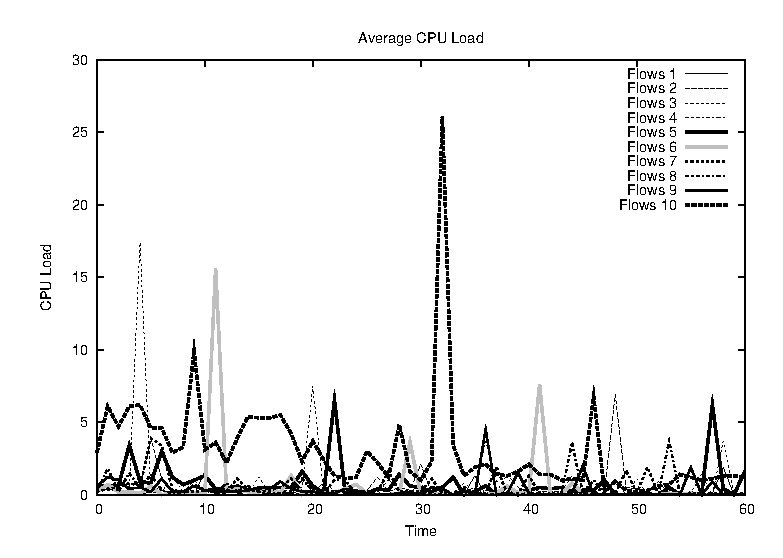
\includegraphics{ScenarioEnergyPlacementDirectBusyMachines-30-m5/cpuload.eps}
\caption{cpuload.eps}\label{fig:cpuload}
\end{figure}

\clearpage
\subsection{Memory State}

\begin{figure}[ht]
\centering
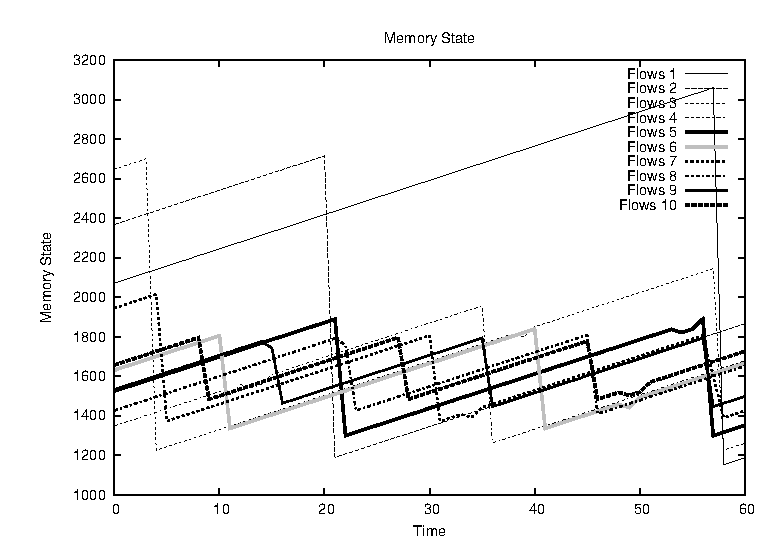
\includegraphics{ScenarioEnergyPlacementDirectBusyMachines-30-m5/memorystorage.eps}
\caption{memorystorage.eps}\label{fig:memorystorage}
\end{figure}

\clearpage
\subsection{Response Time}

\begin{figure}[ht]
\centering
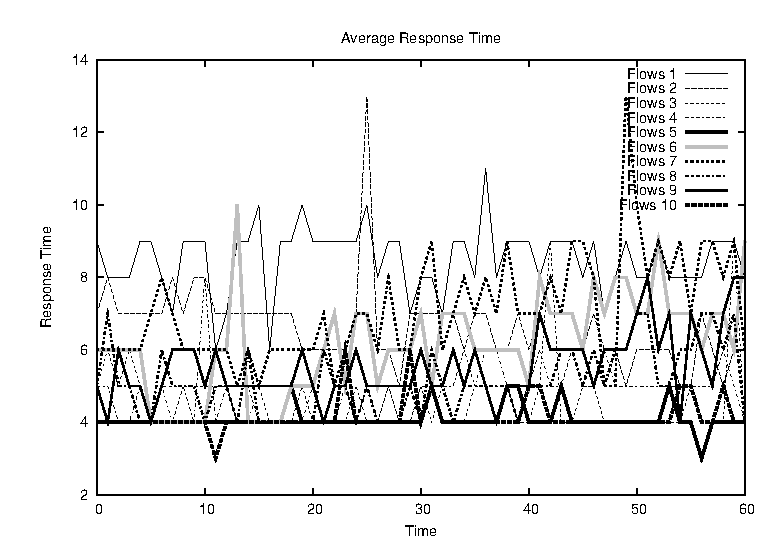
\includegraphics{ScenarioEnergyPlacementDirectBusyMachines-30-m5/responsetime.eps}
\caption{responsetime.eps}\label{fig:responsetime}
\end{figure}

\clearpage
\subsection{Information Freshness}

\begin{figure}[ht]
\centering
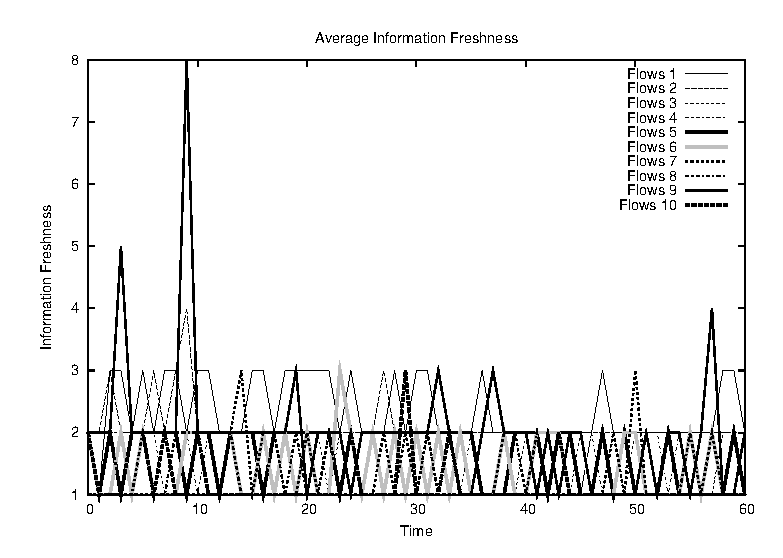
\includegraphics{ScenarioEnergyPlacementDirectBusyMachines-30-m5/freshness.eps}
\caption{freshness.eps}\label{fig:freshness}
\end{figure}

\clearpage
\subsection{Minimum Energy Consumed}

\begin{figure}[ht]
\centering

\includegraphics{ScenarioEnergyPlacementDirectBusyMachines-30-m5/minenergy.eps}
\caption{minenergy.eps}\label{fig:minenergy}
\end{figure}

\clearpage
\subsection{Maximum Energy Consumed}

\begin{figure}[ht]
\centering

\includegraphics{ScenarioEnergyPlacementDirectBusyMachines-30-m5/maxenergy.eps}
\caption{maxenergy.eps}\label{fig:maxenergy}
\end{figure}

\clearpage
\subsection{Average Energy Consumed}

\begin{figure}[ht]
\centering

\includegraphics{ScenarioEnergyPlacementDirectBusyMachines-30-m5/averageenergy.eps}
\caption{averageenergy.eps}\label{fig:averageenergy}
\end{figure}

\clearpage
\subsection{Total Energy Consumed}

\begin{figure}[ht]
\centering

\includegraphics{ScenarioEnergyPlacementDirectBusyMachines-30-m5/totalenergy.eps}
\caption{totalenergy.eps}\label{fig:totalenergy}
\end{figure}

\clearpage
\subsection{Flow Types:Placement EnergyLinear}

\begin{figure}[ht]
\centering
\includegraphics{ScenarioEnergyPlacementDirectBusyMachines-30-m5/flowtypes-0.eps}
\caption{flowtypes-0.eps}\label{fig:flowtypes-0}
\end{figure}

\clearpage
\subsection{Flow Types:Placement EnergyPaper}

\begin{figure}[ht]
\centering
\includegraphics{ScenarioEnergyPlacementDirectBusyMachines-30-m5/flowtypes-1.eps}
\caption{flowtypes-1.eps}\label{fig:flowtypes-1}
\end{figure}

\clearpage
\subsection{Flow Types:Placement EnergyTranscritical}

\begin{figure}[ht]
\centering
\includegraphics{ScenarioEnergyPlacementDirectBusyMachines-30-m5/flowtypes-2.eps}
\caption{flowtypes-2.eps}\label{fig:flowtypes-2}
\end{figure}

\clearpage
\subsection{Flow Types:Placement EnergyPichfork}

\begin{figure}[ht]
\centering
\includegraphics{ScenarioEnergyPlacementDirectBusyMachines-30-m5/flowtypes-3.eps}
\caption{flowtypes-3.eps}\label{fig:flowtypes-3}
\end{figure}

\clearpage
\subsection{Flow Types:Placement LeastBusy}

\begin{figure}[ht]
\centering
\includegraphics{ScenarioEnergyPlacementDirectBusyMachines-30-m5/flowtypes-4.eps}
\caption{flowtypes-4.eps}\label{fig:flowtypes-4}
\end{figure}

\clearpage
\subsection{Flow Types:Placement LeastUsed}

\begin{figure}[ht]
\centering
\includegraphics{ScenarioEnergyPlacementDirectBusyMachines-30-m5/flowtypes-5.eps}
\caption{flowtypes-5.eps}\label{fig:flowtypes-5}
\end{figure}

\clearpage
\subsection{Response Time of Selected Flows}

\begin{figure}[ht]
\centering
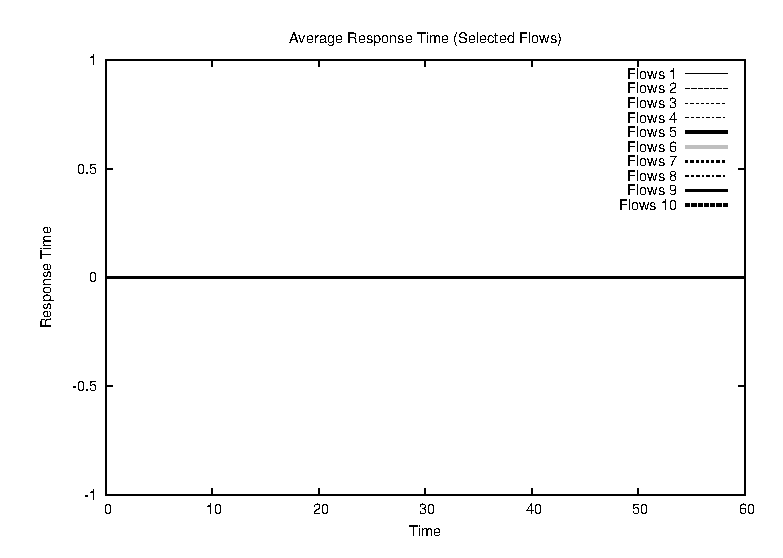
\includegraphics{ScenarioEnergyPlacementDirectBusyMachines-30-m5/responsetimemonitoredflows.eps}
\caption{responsetimemonitoredflows.eps}\label{fig:responsetimemonitoredflows}
\end{figure}

\clearpage
\subsection{Information Freshness of Selected Flows}

\begin{figure}[ht]
\centering
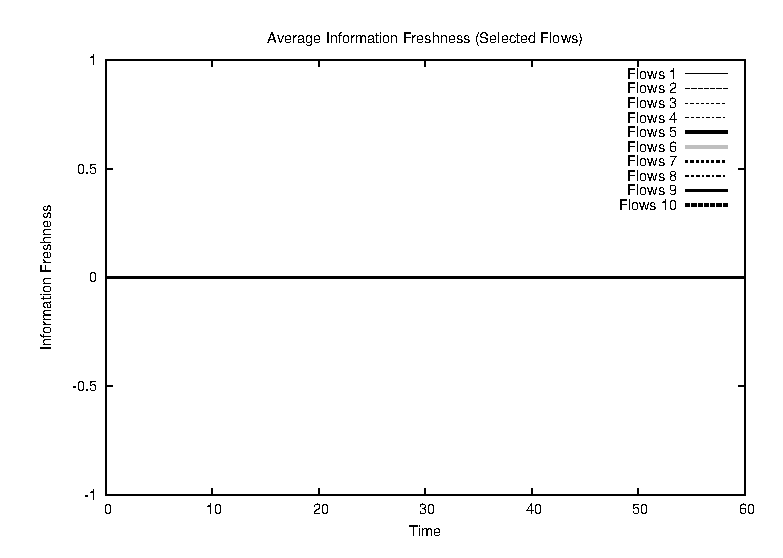
\includegraphics{ScenarioEnergyPlacementDirectBusyMachines-30-m5/freshnessmonitoredflows.eps}
\caption{freshnessmonitoredflows.eps}\label{fig:freshnessmonitoredflows}
\end{figure}

\clearpage

\end{document}
